\section{Автоматизация процессов}

\begin{quote}
\sffamily Под автоматизацией процессов будем понимать набор действий по сборке программного продукта (backend, frontend), действий по управлению  сервисами (останов, запуск, перезапуск), действий по работе с конфигурационными файлами используемых программ и действий по обновлению версий микросервисов, сайта и прочее.
\end{quote}


\subsection{Автоматизация сборки микросервисов}

Много действий по разработке ПО связано с постоянными изменениями в коде, его дополнении и тестировании. Поэтому очень часто приходится пересобирать из исходного кода часть программного продукта. Особенно часто обращает на себя внимаение Backend с его микросервисами. 

Для достижения цели конечного продукта используется 2 сервера: отладочный и производственный. Цели отладочного сводятся непосредственно к разработке ПО, ее отладке и тестированию. Финальную версию ПО выкладывают на производственный сервер, где клиенты пользуются сервисом, пока на отладочном происходит разработка новой версии программного продукта.

Ниже приводится автоматический алгоритм, используемый в текущем проекте:

\begin{enumerate}
	\item Проверка наличия и синтаксиса конфигурационного файла.
	\item Обновление Исходного кода из удаленного репозитория.
	\begin{enumerate}
		\item Проверка текущей ветки;
		\item Обновления копии локального репозитория из удаленной ветки.
	\end{enumerate}
	\item Обновление и модификация UPP\footnote{U ++ --- это кроссплатформенная среда быстрой разработки приложений на C ++, ориентированная на производительность труда программистов. Он включает в себя набор библиотек (GUI, SQL и т.д.) И интегрированную среду разработки.}.
	\begin{enumerate}
		\item Сброс локального репозитория до первоначального состояния;
		\item Обновление из официального репозитория;
		\item Наложение патчей, подготовленных программистами микросервисов в отдельной локальной ветке.
	\end{enumerate}
	\item Выполнение сборки микросервисов.
	\begin{enumerate}
		\item Проверка разрешения на пересборку конкретного микросервиса.
		\item Выполнение сборки проекта микросервиса с помощью встроенного во фреймворк UPP инструмента umk. При сборке указываются необходимые для сборки каждого микросервиса флаги и ключи сборки, конечный путь для новых собранных бинарных файлов.
		\item Установка метки статуса сборки в скрытый временный файл;
		\item Сохранение старой версии микросервиса в файл в постфиксом '.old' в директорию с микросервисом.
	\end{enumerate}
	\item Вызов модуля тестирования микросервисов
	\begin{enumerate}
		\item Проверка статуса сборки;
		\item Вызов модуля UNIT тестов;
		\item Вызов модуля регрессионного тестирования.
	\end{enumerate}
	\item Корректное завершение процессов.
	\begin{enumerate}
		\item Проверка статусов тестирования;
		\item Проверка разрешения на перезапуск микросервиса;
		\item Чтение из конфигурационного файла переменной, содержащей максимальное время ожидания программного завершения микросервиса;
		\item Отправка процессу программного сигнала завершения SIGINT и старт таймера;
		\item Ожидание завершения. Отправка SIGKILL, если процесс не успел завершиться за указанный интервал времени;
		\item Проверка закрытия сетевых портов;
		\item Установка метки статуса сокета, на котором работал микросервис;
	\end{enumerate}
	\item Запуск микросервисов и проверка их состояния.
	\begin{enumerate}
		\item Проверка статуса сетевого порта;
		\item Запуск и демонизация\footnote{Демонизацией процесса называют запуск программы для работы в специальном фоновом режиме даже если пользователь выйдет из системы.} микросервиса;
		\item Ожидание некоторого времени и проверка состояния процесса.
	\end{enumerate}
\end{enumerate}


\subsection{Автоматизация перезапуска микросервисов}

Для реализации перезапуска микросервисов потребовался отдельный скрипт, который отвечает за передачу сигнала прерывания в микросервис и обработку реакции останавливаемой программы на сигнал.
Общий алгоритм останова и перезапуска микросервиса в автоматическом режиме следующий:
\begin{enumerate}
 	\item Проверка разрешения на перезапуск, отмеченным в конфигурационном файле.
 	\item Проверка наличия рабочих процессов микросервиса в системе.
 	\item Отправка сигнала SIGINT на программное завершение.
 	\item Ожидание корректного завершения микросервиса и всех его дочерних процессов в течение указанного в конфигурационном файле времени. Если процесс не завершился самостоятельно, производится отправка сигнала принудительного завершения SIGKILL.
 	\item Ожидание закрытия сетевого порта микросервиса. Если порт не закрывается в течение указанного времени (10 секунд), то автосборка отражает это состояние в параметре статуса порта. 
 	\item Проверка состояние сетевого порта по флагу. Если порт не был закрыт, то процесс автосборки завершается с определенным кодом. 	
\end{enumerate}

Алгоритм ручного перезапуска вызывается в режиме '-restart' и аналогичен автоматическому. Алгоритмы останова и запуска требуют каждый проверку порта, для этого и введен параметр состояния порта. Это необходимо для гарантированного завершения микросервиса. 
Реализованный механизм останова и запуска микросервиса достаточно гибкий, так как включает в себя несколько проверок. Это позволяет максимально корректно завершить работу микросервиса, в каком бы он состоянии не находился.


\subsection{Автоматизация замены версии микросервисов}

Процесс замены версий на отладочном и производственном серверах отличается. Любая сборка проекта происходит на отладочном сервере. В данном случае, как и в случае с автоматизацией сборки и перезапуска микросервисов, учавствует специльно реализованная программа. На отладочном сервере для замены версии микросервисов можно воспользоваться этой утилитой для сборки. Так она перезапишет локальные версии программ. С производственным сервером немного сложнее, так как нужно локально собрать ПО и доставить его. Алгоритм можно описать так:
\begin{enumerate}
	\item Проверка наличия и синтаксиса конфигурационного файла автосборки
	\item Проверка существования бинарных файлов и формирование их списка
	\item Установление SSH соединения с боевым сервером
	\item Остановка микросервисов, используя тот же алгоритм автосборки
	\item Создание бэкапа каждого микросервиса
	\item Перезапись старых бинарных файлов новыми
	\item Запуск микросервисов
	\item Разрыв SSH соединения
\end{enumerate}
На производственном сервере существует две версии одновременно работающих Backend: Beta\footnote{Бета-версия продукта. Используется для предрелиза продукта. В очередной раз команда убеждается, что все работает корректно.} и Production\footnote{Конечый вариант продукта, доступный для использования клиентам.}. Рис. \ref{img:updating} показывает нагладное отношение объектов и последовательность обновления микросервисов.

\begin{figure}[H]
\centering
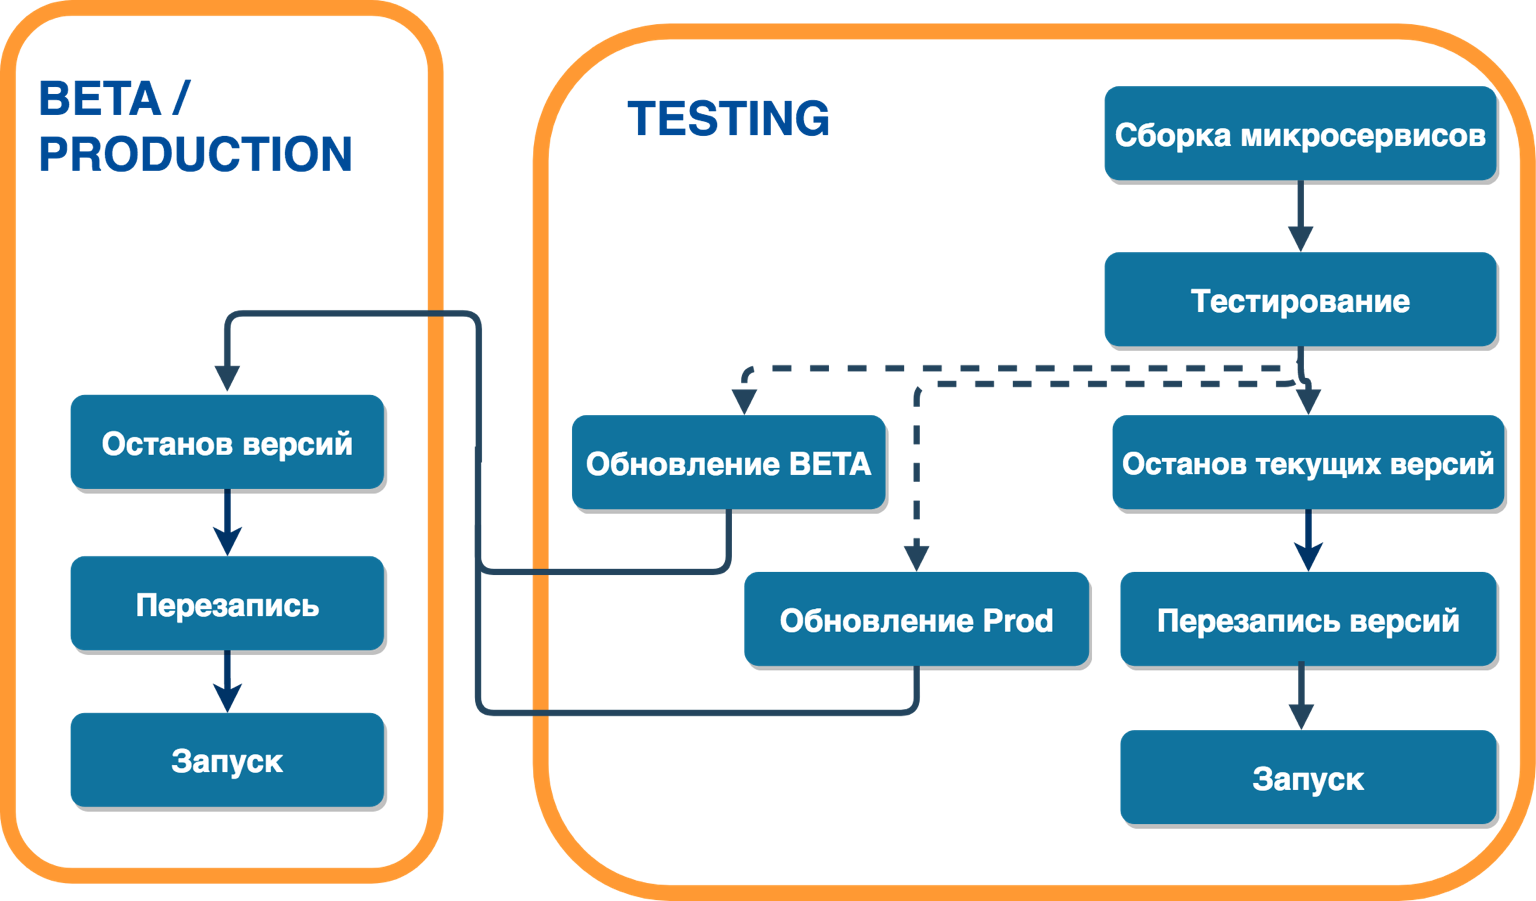
\includegraphics[scale=0.6]{updating.png}
\caption{Схема замены версий на серверах}
\label{img:updating}
\end{figure} 


\subsection{Автоматизация создания доменного имени}

Доменное имя - это самый высокоуровневый атрибут экосистемы клиента. Именно он является визуальной составляющей точки входа в систему, т.е. клиент его видет самым первым в строке браузера. Более того, доменное имя является основной характеристикой экосистемы. Все низлежащие уровни модели сервера оперируют этим именем, а на уровне ДНС-сервера обепечивается "открытие ворот" в систему для клиента. 

Необходимой задачей является добавление нового доменного имени или удаление старого. Домен второго уровня, например, {\ttfamily ingipro.com} является основным для сервиса. Домены третьего уровня являются уникальными для каждой компании, например, {\ttfamily beta.ingipro.com} или {\ttfamily new-company.ingipro.com}. Вот эти домены и предстоит добавлять и удалять из доменной зоны, чтобы открыть или закрыть доступ к сервису для клинета.

Чтобы вручную это сделать, необходимо выполнить слудующие действия:
\begin{enumerate}
	\item Развернуть и настроить ДНС-сервер.
	\item Добавить доменное имя в файл зоны.
	\item Инкриментировать идинтификационный номер файла доменной зоны.
	\item Сохранить изменения.
	\item Выполнить команду ДНС-сервера на чтение нового файла доменной зоны.
	\item Проверить доступность нового доменного имени.
\end{enumerate}
В жизни это окажется рутинной работой, утомительной и неэффективной, а так же велика вероятность ошибиться. Поэтому для этой цели реализуется специальный сценарий, реализующий вышеперечисленные действия, причем с дополнительными проверками синтакисиса и кодов завершения команд.


\subsection{Автоматизации регистрации нового пользователя}

Новый пользователь - клиент, представляет собой некую организацию. Создание точки входа сопровождается созданием экосистемы, в рамках которой клиент будет работать. 
Регистрация экосистемы происходит с помощью API\footnote{API (программный интерфейс приложения, интерфейс прикладного программирования) (англ. application programming interface) --- описание способов (набор классов, процедур, функций, структур или констант), которыми одна компьютерная программа может взаимодействовать с другой программой.}, реализованного командой разработчиком микросервисов.

В процессе регистрации пользователя, а именно в процессе создания экосистемы, учавствуют все уровни архитектуры сервера. Первое~--- это ДНС-сервер. С помошью полученной выше утилиты мы регистрируем доменное имя. Второе~--- база данных PostgreSQL. Роль базы данных состоит в хранении данных в структурированном табличном виде. Третья составляющая~--- это веб-сервер Nginx. Четвертый компонент~--- это один из микросервисов. Он отвечает за авторизацию пользователей в системе, а также за контроль доступа к запрашиваемым данным любого типа и их изменение.

Чтобы зарегистрировать новую экосистему, необходимо создать суперпользователя для экосистемы, далее получить ключ для этого пользователя, а затем уникальный одноразовый номер для создания узла. Каждый HTTP-запрос формируется с помощью утилиты curl, содержащей в качестве аргументов синтаксис API. Затем он отправляется через сокет на порт, на котором работает веб-сервер. Nginx обрабатывает запрос и передает данные в соответствующий микросервис. Этот микросервис выполняет требуемый запрос веб-сервера, используя базу данных, и передает данные веб-серверу, а он клиенту. Так мы получаем метаданные данные. В итоге имеем зарегистрированную экосистему с пользователями для клиента.

Задачей автоматизации является мгновенное создание экосистемы для организации, а также ее изменение, если необходимо добавить или удалить пользователей. При этом необходимо реализовать удобное взаимодействие с процессом регистрации при помощи JSON-файла и файлом с данными экосистемы. 
Для этих целей реализован скрипт на языке Bash. Входным параметром для него является файл экосистемы, названный по доменному имени в формате RFC 1033. Выходными данными является файл формата JSON, содержащий ключ пользователя root, название и список всех пользователей экосистемы с собственными ключами.

Алгоритм работы утилиты регистрации экосистемы следующий:
\begin{enumerate}
	\item Проверка наличия файла экосистемы, имеющего название организации.
	\item Проверка наличия выходного файла JSON с ключами пользователей.
	\item Если такого файла нет, происходит создание экосистемы с нуля.
	\item Если уже имеется конечный JSON файл, тогда происходит добавление или удаление пользователей в зависимости от того, как мы меняем входной файл экосистемы.
	\item Вызов скрипта управления файлом доменной зоны с ключом добавления домена. Если домен не существует, то он добавляется в файл зоны DNS-сервера.
	\item Вывод полученных уникальных ключей пользователей для авторизации в системе Ingipro.
\end{enumerate}
